\section{لیست سیاه}
در این ویژگی، یک لیست‌ سیاه
\lf{Blacklist}
از مکان‌هایی در شبکه وجود دارد که نباید در شبکه به آن‌ها دسترسی وجود داشته باشد
\cite{network-abstractions}
مهم‌ترین استفاده از لیست سیاه را می‌توان برای اعمال سیاست‌های کنترل دسترسی در نظر گرفت که مثلا برخی از هاست‌ها که دارای اطلاعات حیاتی هستند در لیست سیاه قرار می‌گیرند تا از بیرون به آن‌ها دسترسی وجود نداشته باشد.
به عنوان مثال دیگر ممکن است برخی از عناصر شبکه برای تعمیر برای مدتی کنار گذاشته شوند برای این منظور می‌توان آن‌ها را در لیست سیاه قرار داد تا دسترسی به آن‌ها سبب از دست رفتن بسته‌ها نشود.
\begin{figure}
    \centering
    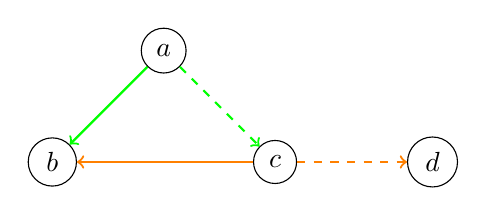
\begin{tikzpicture}[
            node distance={20mm},
            main/.style = {draw, circle},
            s/.style = {->,thick},
            d/.style = {->,thick,dashed} ]
        \node[main] (b) {$b$};
        \node[main] (a) [above right of=b] {$a$};
        \node[main] (c) [below right of=a] {$c$};
        \node[main] (d) [right of=c] {$d$};
        \draw[thick,green,->] (a) -- (b);
        \draw[thick,green,->,dashed] (a) -- (c);
        \draw[thick,orange,->] (c) -- (b);
        \draw[thick,orange,->,dashed] (c) -- (d);
    \end{tikzpicture}
    \caption{ }
    \label{fig:blacklist}
\end{figure}
برای پیدا کردن علت نقض شدن ویژگی لیست سیاه شبکه‌ی رسم شده در شکل
\ref{fig:blacklist}
را در نظر بگیرید.
در این شبکه سوییچ
$d$
در لیست‌ سیاه قرار دارد، بنابراین در هیچ لحظه نباید از
$a$
که ورودی شبکه است در دسترس باشد.
در شبکه‌ی بالا ابتدا مسیر‌هایی که با خط پررنگ مشخص شده‌اند وجود دارند.
در ادامه هر یک از مسیرها با مسیر‌های خط‌چین جایگزین می‌شوند.
فرض کنید به روز رسانی این مسیر‌ها توسط دو پردازه هم‌روند انجام می‌شود.
واضح است که اگر هر دوی این به‌روز رسانی‌ها انجام شوند دسترسی به سوییچی که در لیست سیاه قرار دارد ممکن می‌شود.
اکنون فرض کنید که از عبارات زیر برای توصیف این شبکه در نت‌کت پویا استفاده کنیم:
\begin{equation*}
    \begin{aligned}[c]
        P   & = p!1                             \\
        Q   & = q!1                             \\
        N   & = F \oplus p?1;N_p \oplus q?1;N_q \\
        N_p & = F_p \oplus q?1;F_{pq}           \\
        N_q & = F_q \oplus p?1;F_{pq}           \\
        F   & = a\ra b \oplus c\ra b            \\
    \end{aligned}
    \qquad\qquad
    \begin{aligned}[c]
        F_p         & = a\ra c \oplus c\ra b \oplus a\ra b \\
        F_q         & = a\ra b \oplus c\ra d               \\
        F_{pq}      & = a\ra c \oplus c\ra d \oplus a\ra d \\
        SDN         & = \delta_{\mathcal{L}} (N
        \parallel P \parallel Q)                           \\
        \mathcal{L} & = \s{p!1,p?1,q?1,q?1}                \\
    \end{aligned}
\end{equation*}
در توصیف بالا پردازه‌های
$P$
و
$Q$
به ترتیب وظیفه‌ای ارسال پیام برای به روز رسانی مسیر‌های سبز و نارنجی را دارند.
پردازه‌ی
$N$
رفتار ابتدایی شبکه و پردازه‌های
$N_p$
و
$N_q$
به ترتیب رفتار شبکه را پس از به روز رسانی مسیر‌های سبز و نارنجی توصیف می‌کنند.
پردازه‌ های
$F,F_p,F_q,F_{pq}$
رفتار های ارسالی
\lf{Forwarding}
شبکه را توصیف می‌کنند.
در نهایت رفتار کلی شبکه توسط پردازه‌ی
$SDN$
توصیف شده است که حاصل ترکیب موازی پردازه‌های
$N,P,Q$
و جلوگیری از اجرای عملیات‌های همگام نشده است.
\begin{figure}
    \centering
    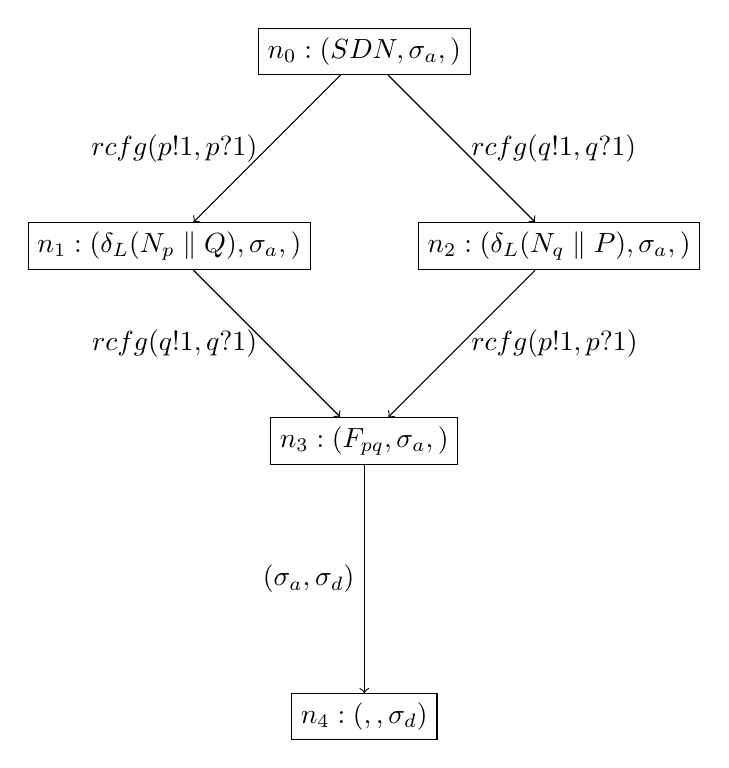
\begin{tikzpicture}[node distance={35mm},
            s/.style = {draw, rectangle,minimum width=5mm} ]
        \node[s] (n0) {$n_0: (SDN,\sigma_a,\his{})$};
        \node[s] (n1) [below left of=n0]
        {$n_1: (\delta_{\mc{L}}(N_p \parallel Q),\sigma_a,\his{})$};
        \node[s] (n3) [below right of=n1]
        {$n_3: (F_{pq},\sigma_a,\his{})$};
        \node[s] (n4) [below of=n3]
        {$n_4:(\checkmark,\his{},\sigma_d)$};
        \node[s] (n2) [below right of=n0]
        {$n_2: (\delta_{\mc{L}}(N_q \parallel P),\sigma_a,\his{}$)};
        \draw[->] (n0) -- node[left]{$rcfg(p!1,p?1)$} (n1);
        \draw[->] (n0) -- node[right]{$rcfg(q!1,q?1)$} (n2);
        \draw[->] (n1) -- node[left]{$rcfg(q!1,q?1)$} (n3);
        \draw[->] (n2) -- node[right]{$rcfg(p!1,p?1)$} (n3);
        \draw[->] (n3) -- node[left]{$(\sigma_a,\sigma_d)$} (n4);
    \end{tikzpicture}
    \caption{}
    \label{fig:blacklist:lts}
\end{figure}
در توصیف بالا امکان اجرای هر دو به روز رسانی وجود دارد
بنابراین شبکه این امکان را دارد که به حالتی برسد که مسیر ارسال
$ad$
در آن وجود داشته باشد.
برای مثال فرض کنید که
$\sigma_a$
یک بسته وارد شده به شبکه باشد که داشته باشیم:
$\sigma_a(sw) = a$.
شکل
\ref{fig:blacklist:lts}
بخشی از نمودار سیستم حالت این شبکه را زمانی که این بسته به شبکه وارد شود نشان می‌دهد.
اگر فرض کنیم
$\sigma_d$
بسته‌ای باشد که
$\sigma_d(sw) = d$
همانطور که در نمودار مشخص است دو مسیر به حالتی که بسته از سوییچ
$a$
به
$d$
برسد وجود دارد.
همانطور که در نمودار مشخص است به دلیل هم‌روندی پردازه‌های
$P$
و
$Q$
دو ترتیب برای اجرای این به‌روز رسانی‌ها وجود دارد و به همین دلیل دو مسیر منجر به خطا در این شبکه وجود دارد.
اکنون می‌خواهیم علت بروز این خطا را پیدا کنیم.
فرض کنید
$\mr{E} = \sem{SDN}$
ساختمان رویداد این شبکه و
$\mc{M}$
مدل علی
$\mr{E}$
بر اساس تعریف
باشد.
در این مدل تابع متغیر
$PV$
را به صورت زیر تعریف می‌کنیم:
\begin{align*}
    \f{PV} & = \exists c \in \mc{F}(ES(\vec v)). \exists e \in c. l(e) = a\ra d
\end{align*}
تابع بالا رفتار ناامن را به گونه‌ای تعریف می‌کند که مقدار آن در صورتی درست است که پیکر بندی‌ای در ساختمان رویداد وجود داشته باشد که رویدادی با برچسب
$a \ra d$
داشته باشد.
با توجه به ترتیب اجرای به‌روز‌رسانی‌ها در شبکه دو رویداد برای هر یک از عملیات‌های
$rcfg(p!1,p?1),rcfg(q!1,q?1),a \ra d$
در ساختمان رویداد وجود دارد.
فرض کنید برای رویداد‌های مرتبط با این عملیات‌ها شش رویداد
$p_1,p_2,q_1,q_2,ad_1,ad_2$
وجود داشته باشد که برچسب آن‌ها به صورت زیر باشد:
\begin{align*}
    l(p_1) & = rcfg(p!1,p?1) \\
    l(p_2) & = rcfg(p!1,p?1) \\
    l(q_1) & = rcfg(q!1,q?1) \\
    l(q_2) & = rcfg(q!1,q?1) \\
    l(ad_1) & = a \ra d \\
    l(ad_2) & = a \ra d 
\end{align*}

\begin{figure}
    \begin{tikzpicture}[scale=0.8]
        \crd{0}{0}{$\emptyset$}
        \crd[left]{-2}{1}{$\s{p_1}$}
        \crd[left]{-2}{2}{$\s{p_1,q_1}$}
        \crd[left]{-2}{3}{$\s{p_1,q_1,ad_1}$}
        \crd[right]{2}{1}{$\s{q_2}$}
        \crd[right]{2}{2}{$\s{p_2,q_2}$}
        \crd[right]{2}{3}{$\s{p_2,q_2,ad_2}$}
        \draw [ultra thick] (-2,1) -- (-2,2);
        \draw [ultra thick] (-2,2) -- (-2,3);
        \draw [ultra thick] (0,0) -- (2,1);
        \draw [ultra thick] (0,0) -- (-2,1);
        \draw [ultra thick] (2,1) -- (2,2);
        \draw [ultra thick] (2,1) -- (2,3);
    \end{tikzpicture}
    \caption{}
    \label{fig:blacklist:es}
\end{figure}

شکل
\ref{fig:blacklist:es}
قسمتی از نمودار ساختمان رویداد این شبکه را نشان می‌دهد که در آن تمام پیکر‌بندی‌هایی که یکی از رویداد‌های 
$ad_1$
یا
$ad_2$
قابل دسترس باشد.
با استفاده از مدل علی در این مثال می‌توانیم
$C(p_1,q_1) = \F$
را به عنوان یک علت برای نقض ویژگی لیست سیاه بیان معرفی کنیم در صورتی که از
$(C(p_2,q_2),\T,\T)$
به عنوان شاهد استفاده کنیم.
در 
$\mr{E}$
پیکربندی 
$\s{p_1,q_1,ad_1}$
قابل دسترسی است.
بنابراین مقدار
$PV$
صحیح است.
همچنین بین رویداد‌های 
$p_1$
و
$q_1$
تعارضی وجود ندارد پس 
$C(p_1,q_1) = \F$.
بنابراین شرط ۱ در تعریف 
برقرار است.
اکنون فرض کنید که مقدار
$C(p_1,q_1)$
و
$C(p_2,q_2)$
را برابر صحیح قرار دهیم.
در این حالت هیچ یک از پیکر‌بندی‌های 
$\s{p_1,q_1,ad_1}$
و
$\s{p_2,q_2,ad_2}$
دیگر نمی‌توانند عضوی از پیکربندی‌های 
$ES(\vec v)$
در 
$\mc{M}$
باشند.
پس در این حالت مقدار
$PV$
غلط می‌شود بنابراین شرط 
۲.الف برقرار می‌شود.
برای بررسی برقراری شرط ۲.ب
باید فرض کنیم که مقدار
$C(p_1,q_1)$
غلط است.
توجه کنید که در این شرایط پیکربندی
$\s{p_1,q_1,ad_1}$
عضوی از پیکربندی‌های 
$ES(\vec v)$
است و مقدار
$C(p_2,q_2)$
روی این مساله تاثیری ندارد.
همچنین برگرداندن مقادیر بقیه متغیر‌ها به مقدار اولیه آن‌ها باعث حذف 
$\s{p_1,q_1,ad_1}$
از مجموعه‌ی پیکربندی‌ها نمی‌شود بنابراین شرط ۲.ب هم برقرار است.
با توجه به اینکه علت تنها شامل یک جمله است بنابراین شرط مینیمال بودن هم برقرار است.
بنابراین در نهایت می‌توان نتیجه گرفت که 
$C(p_1,q_1)$
یک علت واقعی برای بروز خطا در این شبکه است.
به صورت شهودی اتفاق افتادن هر دوی به روز‌رسانی‌ها علت وقوع خطا در این مثال است که توسط تعریف ارائه شده پیدا شده است.

